\begin{figure}[h!]
    \begin{center}
    \caption{Effects on Public Spending per capita - By Category}\label{fig:b2}
    \begin{subfigure}{0.48\textwidth}
        \caption{\scriptsize Health and Sanitation}\label{fig:b2a}
        \centering
        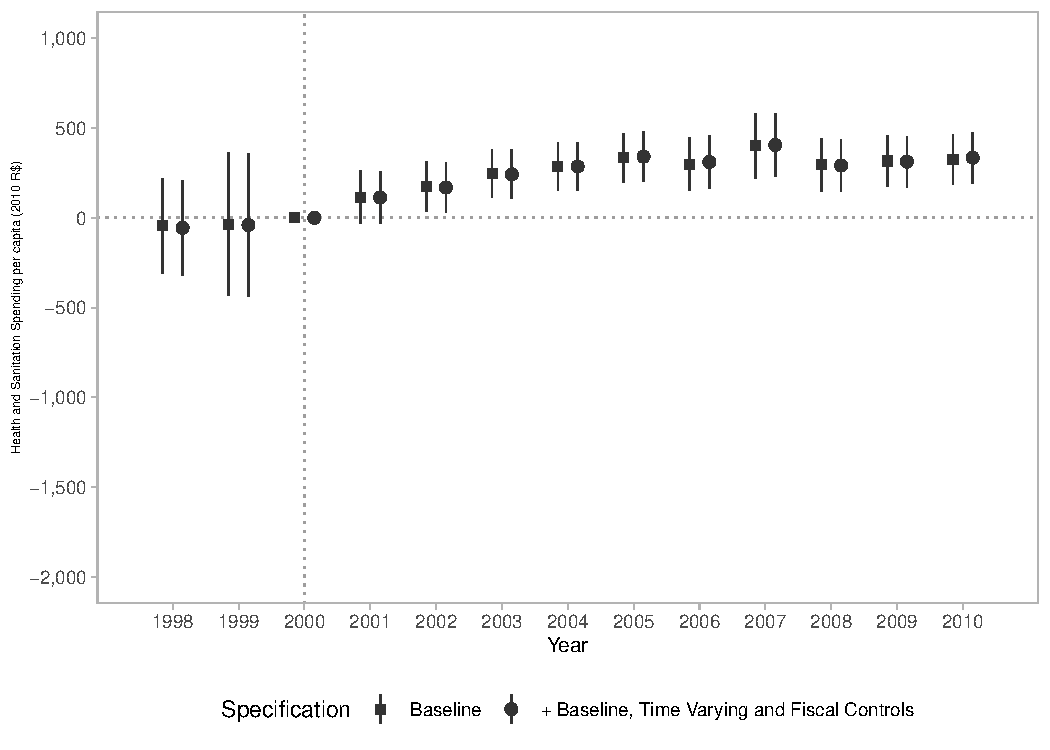
\includegraphics[width=\textwidth]{plots/finbra_desp_saude_san_pcapita_dist_ec29_baseline_dist_ec29_baseline_B2.pdf}
    \end{subfigure}
    \begin{subfigure}{0.48\textwidth}
        \centering
        \caption{\scriptsize Education and Culture}\label{fig:b2b}
        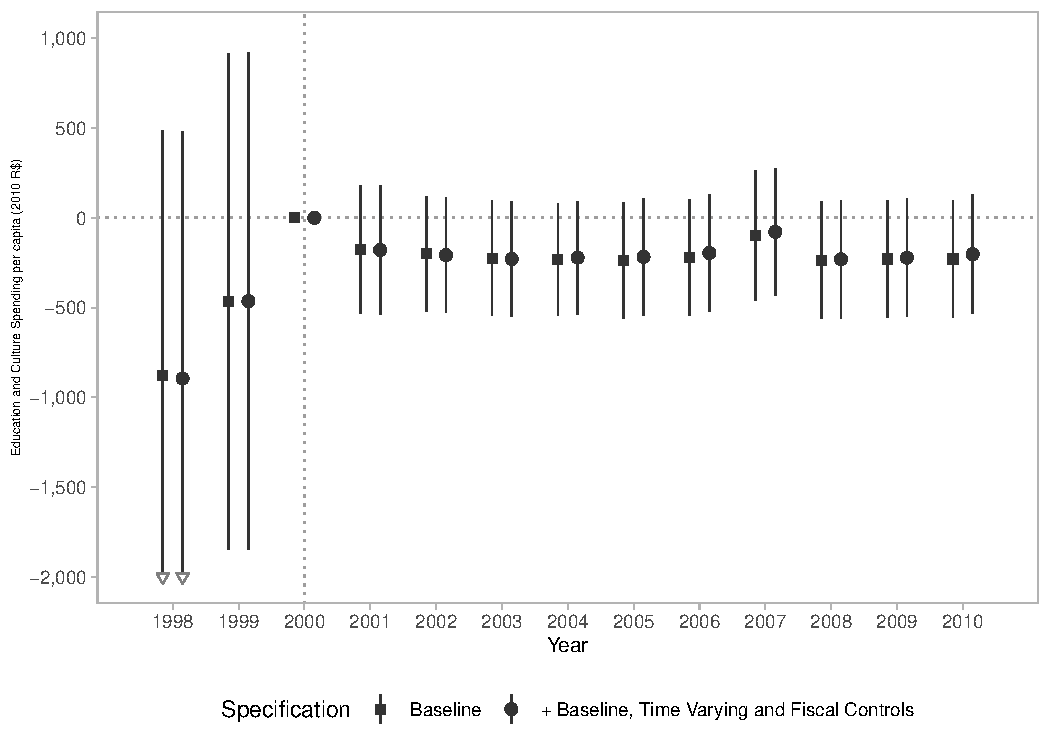
\includegraphics[width=\textwidth]{plots/finbra_desp_educ_cultura_pcapita_dist_ec29_baseline_dist_ec29_baseline_B2.pdf}
    \end{subfigure}
    \begin{subfigure}{0.48\textwidth}
        \centering
        \caption{\scriptsize Social Assistance}\label{fig:b2c}
        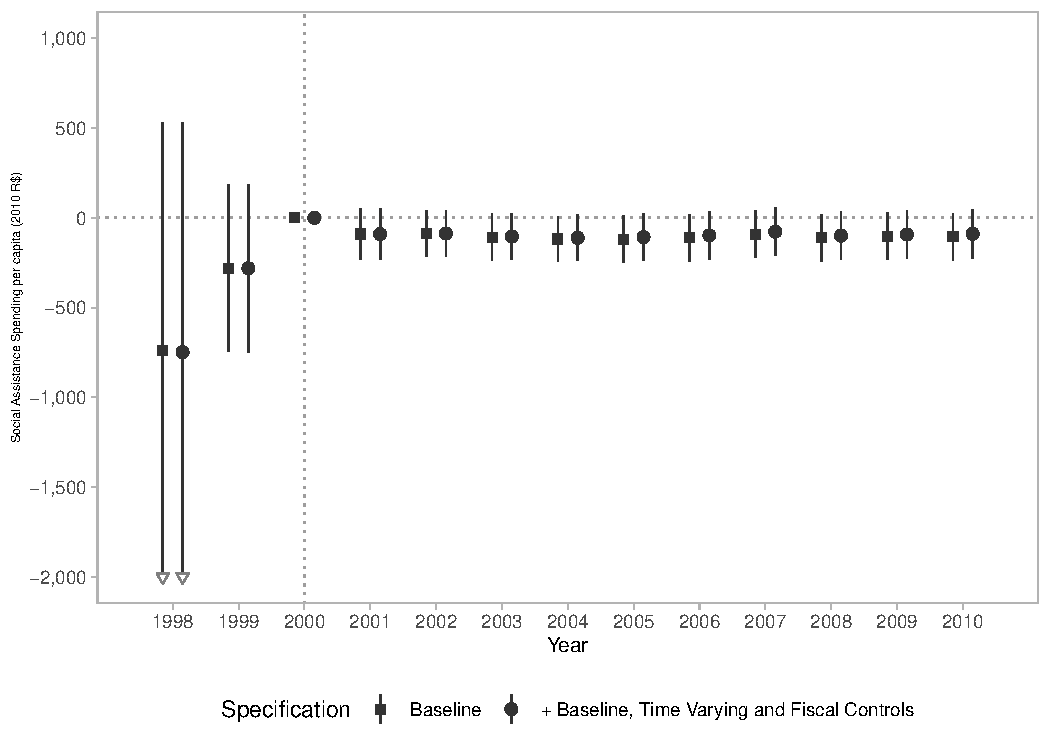
\includegraphics[width=\textwidth]{plots/finbra_desp_assist_prev_pcapita_dist_ec29_baseline_dist_ec29_baseline_B2.pdf}
    \end{subfigure}
    \begin{subfigure}{0.48\textwidth}
        \centering
        \caption{\scriptsize Transport}\label{fig:b2d}
        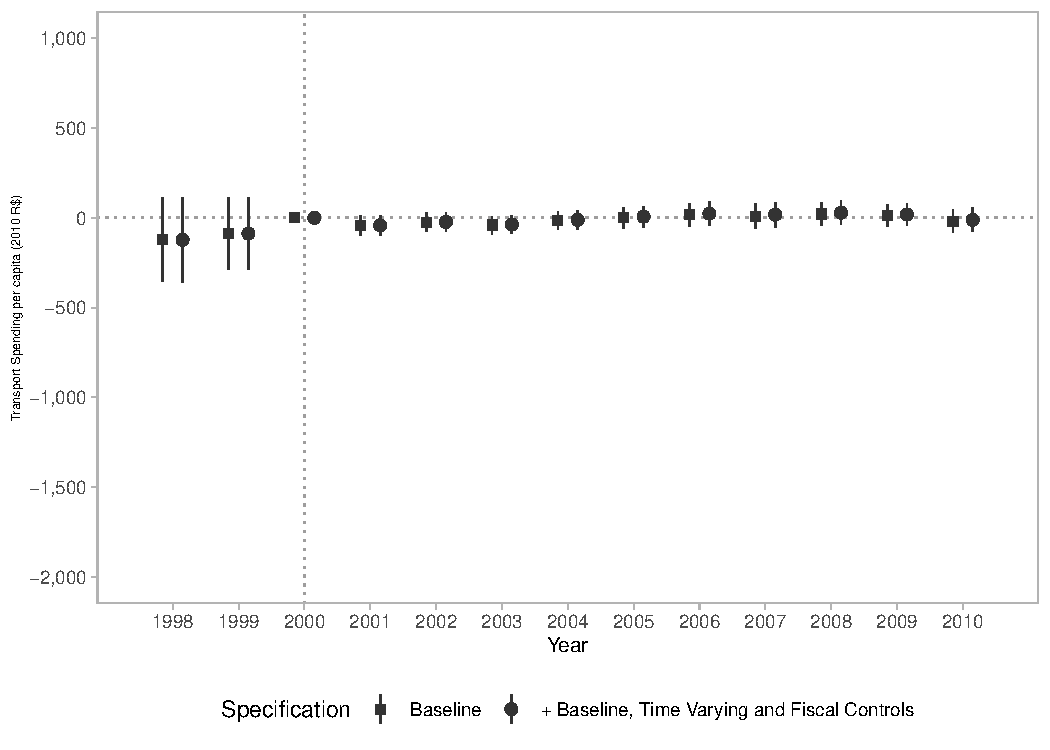
\includegraphics[width=\textwidth]{plots/finbra_desp_transporte_pcapita_dist_ec29_baseline_dist_ec29_baseline_B2.pdf}
    \end{subfigure}
    \begin{subfigure}{0.48\textwidth}
        \centering
        \caption{\scriptsize Housing and Urban}\label{fig:b2e}
        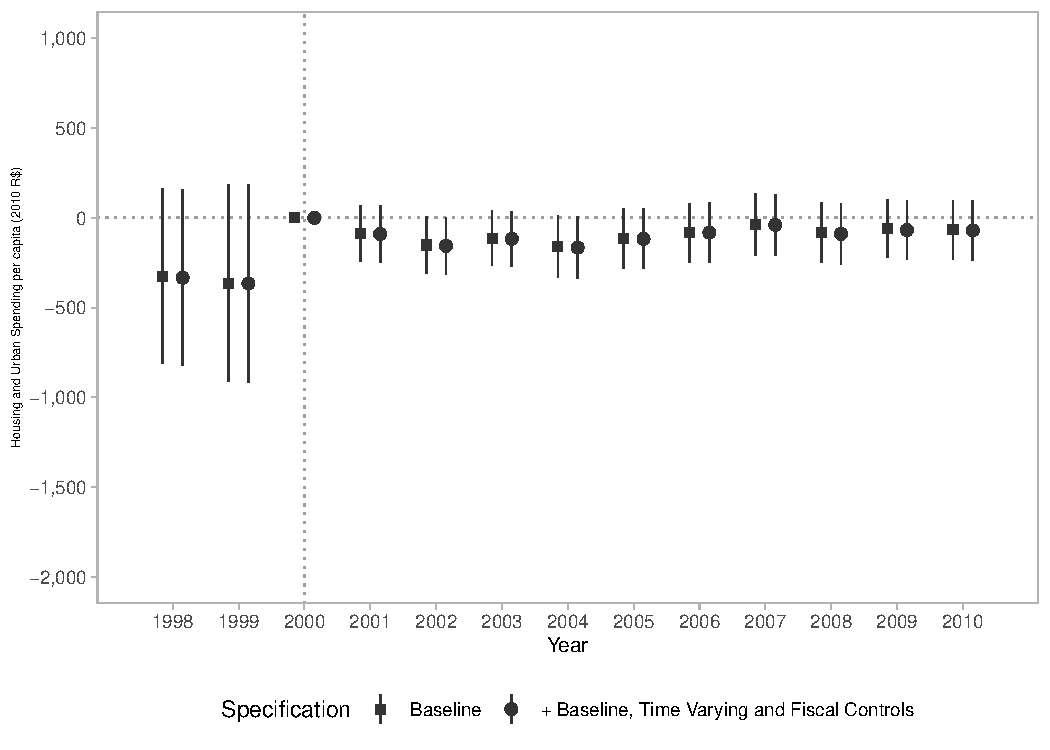
\includegraphics[width=\textwidth]{plots/finbra_desp_hab_urb_pcapita_dist_ec29_baseline_dist_ec29_baseline_B2.pdf}
    \end{subfigure}
    \begin{subfigure}{0.48\textwidth}
        \centering
        \caption{\scriptsize Spending in Other Categories}\label{fig:b2f}
        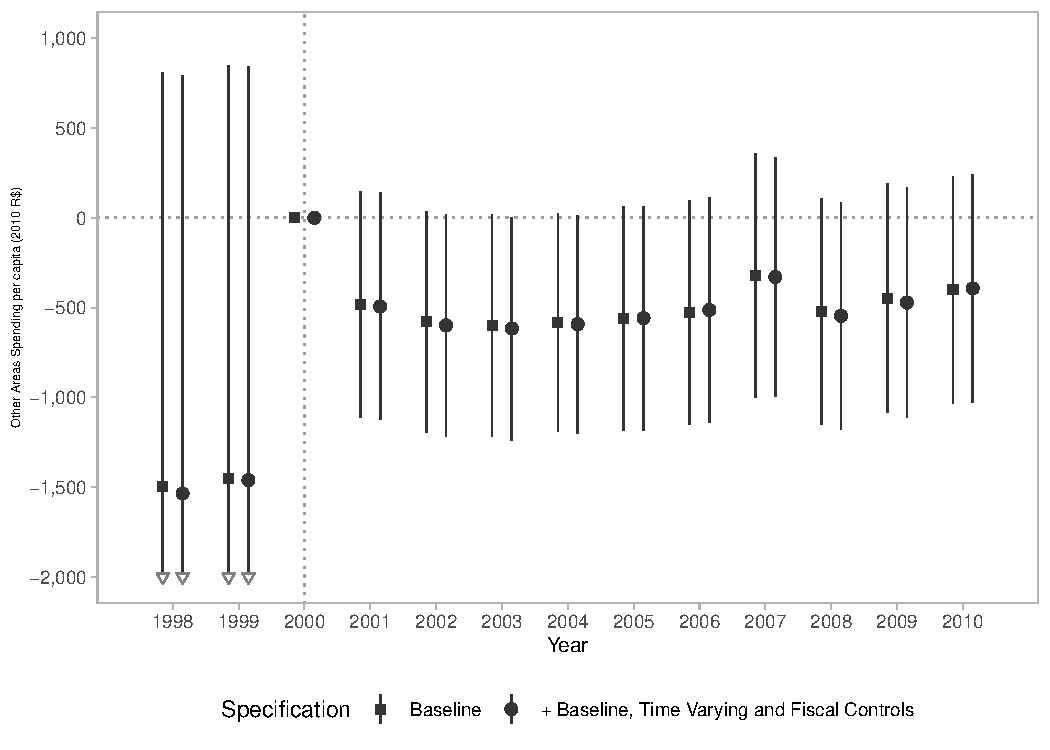
\includegraphics[width=\textwidth]{plots/finbra_desp_outros_area_pcapita_dist_ec29_baseline_dist_ec29_baseline_B2.pdf}
    \end{subfigure}
    
    \end{center}
    \scriptsize{Notes: The number of observations is 64224. DiD Estimates from Equation \ref{eq:2}. Independent variable is the distance to the EC/29 target in p.p. Square dots represent the baseline model with municipality and state-year fixed effects. Round dots represent fully saturated specification (Column 4 in regression Tables). Lines represent 95\% confidence intervals. Arrows, when present, indicate confidence intervals out of the plot bounds. Standard errors are clustered in the municipality level.}
    
\end{figure}